\iffalse
\chapter{2010}
\author{AI24BTECH11004}
\section{ce}

\fi


       \item The inverse of the matrix 
             \begin{align*}
                 \myvec{3+2i & i \\ -i & 3-2i}
             \end{align*}
             is
             \hfill{(2010)}
	       \begin{enumerate}
             \begin{multicols}{2}  
		       \item $\frac{1}{12}\myvec{3+2i & -i \\ i & 3-2i}$
		       \item $\frac{1}{12}\myvec{3-2i & -i \\ i & 3+2i}$
		       \item $\frac{1}{14}\myvec{3+2i & -i \\ i & 3-2i}$
		       \item $\frac{1}{14}\myvec{3-2i & -i \\ i & 3+2i}$
             \end{multicols}
        	\end{enumerate}	
	\item The table below gives values of a function $F(x)$             obtained for values of $x$ at intervals of $0.25$ .
          \begin{align*}
          \begin{tabular}{|l|l|l|l|l|l|}
          \hline$x$ & $0$ & $0.25$ & $0.5$ & $0.75$ & $1.0$ \\
          \hline$\overrightarrow{F}\brak{x}$ & $1$ & $0.9412$ & $0.8$ & $0.64$ & $0.50$ \\
           \hline
           \end{tabular}
           \end{align*}
          The value of the integral of the function between the limits 0 to 1 using Simpson's rule is
          \hfill{(2010)}
               \begin{enumerate}
			        \begin{multicols}{4}  
		       \item $0.7854$
		       \item $2.3562$
		       \item $3.1416$
		       \item $7.5000$
                    \end{multicols}   
	       \end{enumerate}	
       \item The partial differential equation that can be formed from $z=a x+b y+a b$ has the form $\brak{\text{with } p=\frac{\partial z}{\partial x} \text{and } q=\frac{\partial z}{\partial y}}$
       \hfill{(2010)}
		\begin{enumerate}
			\item $z=p x+q y$
			\item $z=p x+p q$
			\item $z=p x+q y+p q$
			\item $z=q y+p q$
		\end{enumerate}
	\item  A parabolic cable is held between two supports at the same level. The horizontal span between the supports is $L$. The sag at the mid-span is $h$. The equation of the parabola is $y=4 h \frac{x^{2}}{L^{2}}$, where $x$ is the horizontal coordinate and $y$ is the vertical coordinate with the origin at the centre of the cable. The expression for the total length of the cable is
	\hfill{(2010)}
		\begin{enumerate}
			\item $\int_{0}^{L} \sqrt{l+64 \frac{h^{2} x^{2}}{L^{2}}} d x$
			\item $2 \int_{0}^{L / 2} \sqrt{1+64 \frac{h^{3} x^{2}}{L^{4}}} d x$
			\item $\int_{0}^{2 / 2} \sqrt{1+64 \frac{h^{2} x^{2}}{L^{4}}} d x$
	        \item $2 \int_{0}^{4 / 2} \sqrt{1+64 \frac{h^{2} x^{2}}{l^{4}}} d x$
        	\end{enumerate}
	\item Given a function 
          \begin{align*}
           f\brak{x, y}=4 x^{2}+6 y^{2}-8 x-4 y+8
           \end{align*}
           The optimal value of $f\brak{x, y}$
           \hfill{(2010)}
		\begin{enumerate}
		       \item is a minimum equal to $10 / 3$
		       \item is a maximum equal to $10 / 3$
		       \item is a minimum equal to $8 / 3$
		       \item is a maximum equal to $8 / 3$
        	\end{enumerate}	
	\item A double cover butt riveted joint is used to connect two flat plates of $200 mm$ width and $14 mm$ thickness as shown in the figure. There are twelve power driven rivets of $20 mm$ diameter at a pitch of $50 mm$ in both directions on either side of the plate. Two cover plates of $10 mm$ thickness are used. The capacity of the joint in tension considering bearing and shear ONLY, with permissible bearing and shear stresses as $300 MPa$ and $100 MPa$ respectively is
	\hfill{(2010)}
		
\centering
\resizebox{0.4\textwidth}{!}{%
\begin{circuitikz}
\tikzstyle{every node}=[font=\small]
\draw (-0.75,17.25) to[short] (10,17.25);
\draw (-0.75,17.25) to[short] (-0.75,12.75);
\draw (-0.75,12.75) to[short] (10,12.75);
\draw (10,17.25) to[short] (10,12.75);
\draw [dashed] (4.25,17.25) -- (4.25,12.75);
\draw [dashed] (4.5,17.25) -- (4.5,12.75);
\draw [dashed] (0.25,17.25) -- (0.25,12.5);
\draw [dashed] (1.25,17.25) -- (1.25,12.75);
\draw [dashed] (2.25,17.25) -- (2.25,12.75);
\draw [dashed] (3.25,17.25) -- (3.25,12.75);
\draw [dashed] (5.5,17.25) -- (5.5,13);
\draw [dashed] (5.5,13) -- (5.5,12.75);
\draw [dashed] (6.75,17.25) -- (6.75,12.75);
\draw [dashed] (7.75,17.25) -- (7.75,12.75);
\draw [dashed] (8.75,17.25) -- (8.75,12.75);
\draw [dashed] (-0.75,16.25) -- (10,16.25);
\draw [dashed] (-0.75,15) -- (10,15);
\draw [dashed] (-0.75,13.75) -- (10,13.75);
\draw  (0.25,16.25) circle (0.25cm);
\draw  (0.25,15) circle (0.25cm);
\draw  (0.25,13.75) circle (0.25cm);
\draw  (1.25,16.25) circle (0.25cm);
\draw  (1.25,15) circle (0.25cm);
\draw  (1.25,13.75) circle (0.25cm);
\draw  (2.25,16.25) circle (0.25cm);
\draw  (2.25,15) circle (0.25cm);
\draw  (2.25,13.75) circle (0.25cm);
\draw  (3.25,16.25) circle (0.25cm);
\draw  (3.25,15) circle (0.25cm);
\draw  (3.25,13.75) circle (0.25cm);
\draw  (5.5,16.25) circle (0.25cm);
\draw  (5.5,15) circle (0.25cm);
\draw  (5.5,13.75) circle (0.25cm);
\draw  (6.75,16.25) circle (0.25cm);
\draw  (6.75,15) circle (0.25cm);
\draw  (6.75,13.75) circle (0.25cm);
\draw  (7.75,16.25) circle (0.25cm);
\draw  (7.75,15) circle (0.25cm);
\draw  (7.75,13.75) circle (0.25cm);
\draw  (8.75,16.25) circle (0.25cm);
\draw  (8.75,15) circle (0.25cm);
\draw  (8.75,13.75) circle (0.25cm);
\node [font=\small] at (0.75,17.5) {50mm};
\node [font=\small] at (-1.25,15.75) {50mm};
\draw [->, >=Stealth] (-1.25,16) -- (-1.25,16.25);
\draw [->, >=Stealth] (-1.25,15.5) -- (-1.25,15);
\end{circuitikz}
}%


		\begin{enumerate}
			\item $1083.6$ kN
			\item $871.32$ kN
			\item $541.8$ kN
			\item $433.7$ kN
        	\end{enumerate}
	\item Two plates, subjected to direct tension, each of $10 mm$ thickness and having widths of $100 mm$ and $175 mm$ , respectively are to be fillet welded with an overlap of $200 mm$ . Given that the permissible weld stress is $110 MPa$ and the permissible stress in steel is $150 MPa$ , the length of the weld required using the maximum permissible weld size as per $IS:800-1984$ is
	\hfill{(2010)}
		\begin{center}
   	\begin{center}
\resizebox{0.5\textwidth}{!}{%
	\begin{circuitikz}\tikzstyle{every node}=[font=\small]
\draw (1.75,19) to[short] (7.75,19);
\draw (7.75,19) to[short] (7.75,14.75);
\draw (1.75,19) to[short] (1.75,17.75);
\draw (0.25,17.75) to[short] (5.25,17.75);
\draw (0.25,17.75) to[short] (0.25,16);
\draw (0.25,16) to[short] (5.25,16);
\draw (5.25,17.75) to[short] (5.25,16);
\draw (1.75,16) to[short] (1.75,14.75);
\draw (1.75,14.75) to[short] (7.75,14.75);
\node [font=\small] at (1.75,17) {100mm};
\node [font=\small] at (3.5,15.75) {200mm};
\node [font=\small] at (7,17) {175mm};
\draw [->, >=Stealth] (1.75,17.25) -- (1.75,17.75);
\draw [->, >=Stealth] (1.75,16.75) -- (1.75,16);
\draw [->, >=Stealth] (3,15.75) -- (2,15.75);
\draw [->, >=Stealth] (4,15.75) -- (5.25,15.75);
\draw [->, >=Stealth] (7,17.25) -- (7,18.75);
\draw [->, >=Stealth] (7,16.75) -- (7,15);
	\end{circuitikz}}%
\end{center}


		\end{center}
		\newpage
		\begin{enumerate}
		       \item $245.3 mm$
		       \item $229.2 mm$
		       \item $205.5 mm$
		       \item $194.8 mm$
        	\end{enumerate}	
	

	\item For the simply supported bearn of length L. subjected to a uniformly distributed moment M kN-m per unit length as shown in the figure, the bending moment $\brak{\text{in } kN-m}$ at the mid-span of the beam is
	\hfill{(2010)}
     	\begin{center}
\resizebox{0.5\textwidth}{!}{%
	\begin{circuitikz}\tikzstyle{every node}=[font=\small]
\draw [short] (1.5,17.75) -- (6.75,17.75);
\draw [short] (1.5,18.25) -- (6.75,18.25);
\draw [short] (1.5,18.25) -- (1.5,17.75);
\draw [short] (6.75,18.25) -- (6.75,17.75);
\draw [short] (1.5,17.75) -- (1,16.75);
\draw [short] (1.5,17.75) -- (2,16.75);
\draw [short] (1,16.75) -- (2,16.75);
\draw [short] (6.75,17.75) -- (6.25,16.75);
\draw [short] (6.75,17.75) -- (7.25,16.75);
\draw [short] (6.25,16.75) -- (7.25,16.75);
\draw  (6.25,16.5) circle (0.25cm);
\draw  (6.75,16.5) circle (0.25cm);
\draw  (7.25,16.5) circle (0.25cm);
\draw [short] (1.25,16.75) -- (1,16.5);
\draw [short] (1.5,16.75) -- (1.25,16.5);
\draw [short] (1.75,16.75) -- (1.5,16.5);
\draw [short] (2,16.75) -- (1.75,16.5);
\draw [short] (1,16.75) -- (0.75,16.5);
\draw [short] (6,16.25) -- (7.5,16.25);
\draw [short] (6,16.25) -- (5.75,16);
\draw [short] (6.25,16.25) -- (6,16);
\draw [short] (6.5,16.25) -- (6.25,16);
\draw [short] (7,16.25) -- (6.75,16);
\draw [short] (6.75,16.25) -- (6.5,16);
\draw [short] (7.25,16.25) -- (7,16);
\draw [short] (7.5,16.25) -- (7.25,16);
\draw [->, >=Stealth] (2.25,18.75) -- (2.25,17.25);
\draw [->, >=Stealth] (3,18.75) -- (3,17.25);
\draw [->, >=Stealth] (3.75,18.75) -- (3.75,17.25);
\draw [->, >=Stealth] (4.5,18.75) -- (4.5,17.25);
\draw [->, >=Stealth] (5.5,18.75) -- (5.5,17.25);
\draw [->, >=Stealth] (3.25,19.25) -- (5.25,19.25)node[pos=0.6, fill=white]{M kN-m per unit length};
\end{circuitikz}
	}%
\end{center}

		\begin{enumerate}
			\item zero
            \item M
            \item ML
            \item M/L
        	\end{enumerate}	
	\item  A disc of radius $r$ has a hole of radius $r / 2$ cut-out as shown. The centroid of the remaining disc \brak{shaded portion} at a radial distance from the centre $"O"$ is
	\hfill{(2010)}
        	\begin{center}
\resizebox{0.5\textwidth}{!}{%
	\begin{circuitikz}\tikzstyle{every node}=[font=\large]
\draw  (3.75,19.25) circle (2.5cm);
\draw  (6.25,19.5) circle (5cm);
\draw [->, >=Stealth] (3.75,19.25) -- (1.25,19);
\draw [->, >=Stealth] (6.25,19.5) -- (11.25,20);
\node [font=\normalsize] at (2.5,19.5) {r/2};
\node [font=\normalsize] at (8.5,20) {r};
\node [font=\large] at (4,19.25) {O'};
\draw [dashed] (3.25,23.5) -- (7.5,24.25);
\draw [dashed] (4,24) -- (6.25,24.5);
\draw [dashed] (2.5,22.75) -- (8.5,23.75);
\draw [dashed] (1.75,21.75) -- (9.25,23.25);
\draw [dashed] (1.5,20.75) -- (1.75,20.75);
\draw [dashed] (4.75,21.5) -- (10,22.75);
\draw [dashed] (5.75,21) -- (10.5,22);
\draw [dashed] (6.25,20) -- (11,21);
\draw [dashed] (6.25,18.75) -- (11.25,19.5);
\draw [dashed] (5.5,17.75) -- (11.25,18.5);
\draw [dashed] (2.75,16.25) -- (10.75,17.5);
\draw [dashed] (3.25,15.25) -- (9.75,16.25);
\draw [dashed] (5,14.75) -- (9,15.5);
\end{circuitikz}}%
\end{center}

		\begin{enumerate}
            \begin{multicols}{2}
			\item $\frac{r}{2}$
			\item $\frac{r}{3}$
			\item $\frac{r}{6}$
			\item $\frac{T}{8}$
   \end{multicols}
        	\end{enumerate}	
	\item A three hinged paribolic arch having a span of $20 m$ and a rise of $5 m$ carries a point load of $10 kN$ at quarter span from the left end as shown in the figure. The resultant reaction at the left support and its inclination with the horizontal are respectively
	\hfill{(2010)}
         	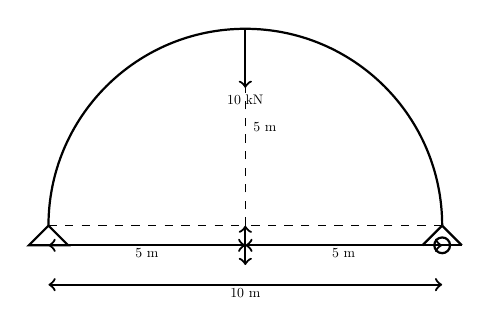
\begin{tikzpicture}[scale=0.5, every node/.style={scale=0.5}]

% Draw the semicircular arch
\draw[thick] (0,0) arc[start angle=180,end angle=0,radius=5];

% Draw supports at the ends of the arch
\draw[thick] (0,0) -- (-0.5,-0.5) -- (0.5,-0.5) -- cycle;  % Left support
\draw[thick] (10,0) -- (9.5,-0.5); % Right support (roller)
\draw[thick] (10,0) -- (10.5,-0.5);
\draw[thick] (9.5,-0.5) -- (10.5,-0.5);
\draw[thick] (10,-0.5) circle (0.2); % Roller circle

% Draw vertical load arrow at the top
\draw[->,thick] (5,5) -- (5,3.5);
\node at (5,3.2) {10 kN};

% Vertical dashed lines from arch to base (distances)
\draw[dashed] (0,0) -- (5,0);
\draw[dashed] (5,0) -- (5,5);
\draw[dashed] (10,0) -- (5,0);

% Draw horizontal dimension lines
\draw[<->,thick] (0,-0.5) -- (5,-0.5);
\node at (2.5,-0.7) {5 m};

\draw[<->,thick] (5,-0.5) -- (10,-0.5);
\node at (7.5,-0.7) {5 m};

\draw[<->,thick] (0,-1.5) -- (10,-1.5);
\node at (5,-1.7) {10 m};

% Draw vertical dimension line
\draw[<->,thick] (5,-1) -- (5,0);
\node at (5.5,2.5) {5 m};

\end{tikzpicture}

                \begin{enumerate}
			\item $9.01 kN$ and $56.31^{\circ}$
			\item $9.01 kN$ and $33.69^{\circ}$
			\item $7.50 kN$ and $56.31^{\circ}$2.50 kN and $33.69^{\circ}$
			\item $2.50 kN$ and $33.69^{\circ}$
        	\end{enumerate}		
	\item The vertical stress at point $P_{1}$ due to the point load $Q$ on the ground surface as shown in figure is $\sigma_{z}$. According to Boussinesq's equation, the vertical stress at point $P_{z}$ shown in figure will be
	\hfill{(2010)}
        	\begin{center}
\resizebox{0.5\textwidth}{!}{%
	\begin{circuitikz}
\tikzstyle{every node}=[font=\large]
\draw [line width=0.5pt, short] (2,28.25) -- (11.25,28.25);
\draw [line width=0.5pt, dashed] (3.75,28.25) -- (3.75,21.75);
\draw [line width=0.5pt, dashed] (3.75,22.25) -- (11,22.25);
\draw [line width=0.5pt, dashed] (3.75,28.25) -- (11,22.25);
\draw [line width=0.5pt, dashed] (3.75,25.5) -- (7.25,25.5);
\draw [line width=0.5pt, <->, >=Stealth] (3.75,21.75) -- (11,21.75);
\draw [line width=0.5pt, <->, >=Stealth] (3,28.25) -- (3,22.25);
\draw [line width=0.5pt, ->, >=Stealth] (3.75,29.25) -- (3.75,28.5);
\node [font=\large] at (3.75,29.75) {Q};
\node [font=\large] at (2.5,25.25) {z};
\node [font=\large] at (7.25,27.25) {z/2};
\draw [line width=0.5pt, dashed] (6.75,28) -- (6.75,26);
\node [font=\large] at (5.25,25.25) {r/2};
\node [font=\large] at (7,21.5) {r};
\node [font=\large] at (7.5,25.75) {P2};
\node [font=\large] at (11.25,22.25) {P1};
\end{circuitikz}
}%

\end{center}

		\begin{enumerate}
			\item $\sigma_{z} / 2$
			\item $\sigma_{z}$
			\item $2 \sigma_{z}$
			\item $4 \sigma_{z}$
        	\end{enumerate}	
	\item An open ended steel barrel of $1 m$ height and $1 m$ diameter is filled with saturated fine sand having coefficient of permeability of $10^{-2} m / s$. The barrel stands on a saturated bed of gravel. The time required for the water level in the barrel to drop by $0.75 m$ is
	\hfill{(2010)}
		\begin{enumerate}
			\item $58.9 s$
			\item $75 s$
			\item $100 s$
			\item $150 s$
        	\end{enumerate}	
	\item The ultimate load capacity of a $10m$ long concrete poilre of square cross section $500 mm x 500 mm $ driven into a homogeneous clay layer having undrained conhesion value of $40kPa$ is $700kN$. If the cross section of the pile is reduced to $250mm x 250mm$ and the length of the pile is increased to $20m $, the ultimate load capacity will be 
	\hfill{(2010)}
		\begin{enumerate}
			\item $350 kN$
			\item $632.5 kN$
			\item $722.5 kN$
			\item $1400 kN$
        	\end{enumerate}	

